\documentclass[hyperref={pdfpagelabels=false}]{beamer}
\usepackage{lmodern}
\usetheme{CambridgeUS}

\usepackage[english,brazilian]{babel}
\usepackage{multicol}
\usepackage{textcomp}
\usepackage[alf]{abntex2cite}
\usepackage[utf8]{inputenc}
\usepackage[T1]{fontenc}
\usepackage{graphicx} %Pacote de imagens
\graphicspath{{./figures/}}

\title{REVISÃO \\ CÁLCULO I}  
\author[Matheus Pimenta]{Matheus Pimenta} 
\institute[UEL]{\normalsize Universidade Estadual de Londrina \\
	Londrina
} 
\date{Fev. 2022} 
\begin{document}
	
\begin{frame}
\titlepage
\end{frame} 


%\begin{frame}
%\frametitle{Table of contents}
%\tableofcontents
%\end{frame} 


\section{Apresentação} 


\begin{frame}
\frametitle{Apresentação} 

Matheus Pimenta \pause

e-mail: matheus.pimenta@outlook.com ou omatheuspimenta@outlook.com \pause

Informações sobre a disciplina \pause

Dúvidas gerais


\end{frame}

\section{REVISÃO - FUNÇÕES}

\begin{frame}
\frametitle{Conjuntos Numéricos}
\begin{itemize}
 \item $\mathbb{N}$ O conjunto $\mathbb{N}$	dos números naturais é caracterizado pelos axiomas de Peano.

    \begin{enumerate}
        \item Todo número natural $n$ tem um sucessor $s(n)$, que ainda é um número natural, números diferentes têm sucessores diferentes. \pause
        \item Existe um único número natural $1$ que não é sucessor de nenhum outro. \pause
        \item Se um conjunto de números naturais contém o $1$ e contém também o sucessor de cada um de seus elementos, então esse conjunto contém todos os números naturais. \pause
    \end{enumerate}

\end{itemize}

\end{frame}

\begin{frame}
\frametitle{Conjuntos Numéricos}

\begin{itemize}
 \item $\mathbb{Z}$: \pause dos números inteiros é definido por: $$\mathbb{Z} = \{ 0, \pm 1, \pm 2, \pm 3, \dots \}$$. \pause
 \item $\mathbb{Q}$: \pause dos números racionais é formado pelas razões de inteiros: $$ \mathbb{Q} = \left\{ \frac{p}{q} ; p,q \in \mathbb{Z} \text{ e } q \neq 0 \right\}$$
\end{itemize}

\end{frame}


\begin{frame}
\frametitle{Conjuntos Numéricos}

\begin{itemize}
 \item $\mathbb{R}$: \pause dos números reais pode ser definido como o conjunto de todas as possíveis expansões decimais. Assim, um número real $a,d_{1}d_{2}d_{3}\dots$ pode ser representado por uma ``soma infinita'' de números racionais: $$a + \frac{d_1}{10} + \frac{d_2}{10^2} + \dots $$
\end{itemize}


\end{frame}

\begin{frame}
\frametitle{Equações}

\begin{itemize}
 \item Equações de 1º Grau: \pause são expressões do tipo $ax+b=0$, com $a \neq 0$, onde $a$ e $b$ são coeficientes da equação e $x$ é a incógnita. \pause
 \item Equações de 2º Grau: \pause são expressões do tipo $ax^{2} + bx + c = 0$, com $a \neq 0$, onde $a,b$ e $c$ são coeficientes e $x$ é a incógnita. Nem sempre possui raízes reais, mas possui uma ou duas raízes em $\mathbb{C}$.
\end{itemize}

\end{frame}

\begin{frame}
\frametitle{Divisão de Polinômios}

Seja $f(x) = a_0x^n+a_1x^{n-1}+\dots+a_{n-1}x+a_n$ e $g(x)=x-a$. 

Se $f(a)=0$, então existe $q(x)=q_0x^{n-1}+q_1x^{n-2}+\dots+q_{n-2}x+q_{n-1}$ tal que $q(x).g(x)=f(x)$.


\end{frame}

\begin{frame}
\frametitle{Funções Reais de uma Variável Real}

Sejam $D$ e $Y$ conjuntos não-degenerados. Uma função $f:D \rightarrow Y$ é uma regra que associa, a cada elemento $x \in D$, um único elemento $f(x) \in Y$. \pause

Função: \pause É uma relação em que todos os elementos $x$ do conjunto $A$, se relacionam uma {\bf única} vez com os elementos $y$ do conjunto $B$, ou seja, $f: A \rightarrow B$, ou ainda, $(f): \mathbb{R} \rightarrow \mathbb{R}$, ou simplesmente $(f): X\rightarrow Y = f(x)$, na prática escrevemos $y = f(x)$. \pause

O conjunto $D$ é denominado domínio da função. O conjunto $Y$ é denominado contra-domínio. A imagem da função $f$ é o conjunto formado por todos os pontos $y \in Y$ tais que existe um $x_0 \in D$ com $f(x_0) = y$. Note que $Im(f) \subset Y$, mas não necessariamente a imagem possui todos os elementos do contra-domínio.
\end{frame}

\begin{frame}
\frametitle{Funções Monótonas}

Uma função $f:D \rightarrow \mathbb{R}$, com $D \subset \mathbb{R}$, chama-se:
\begin{itemize}
	\item não-decrescente, se $x<y \Rightarrow f(x) \leq f(y)$;
	\item não-crescente, se $x<y \Rightarrow f(x) \geq f(y)$;
	\item crescente, se $x<y \Rightarrow f(x) < f(y)$;
	\item decrescente, se $x<y \Rightarrow f(x) > f(y)$.
\end{itemize}

\end{frame}

\begin{frame}
\frametitle{Composição de Funções}
Sejam $A$, $B$ e $C$ conjuntos e sejam as funções $f:A \rightarrow B$ e $g: B \rightarrow C$. A função $ g \circ f : A \rightarrow C$ é definida por:
$$(g \circ f)(x) = g(f(x))$$

Note que $g \circ f$ costuma ser diferente de $ f \circ g$.

\end{frame}

\begin{frame}
\frametitle{Principais Funções Elementares}

\begin{itemize}
 \item Função Polinomial: \pause $$f(x) = a_0+a_1x+a_2x^2+\dots+a_nx^n$$ \pause
 \item Função Racional: \pause $$f(x) = \frac{p(x)}{q(x)},$$ onde $p$ e $q$ são funções polinomiais. O domínio de $f$ é $\{x \in \mathbb{R}; q(x) \neq 0 \}$ \pause
 \item Funções Trigonométricas: \pause $\sin (\alpha) = \displaystyle \frac{b}{a}$ e $\cos(\alpha) = \displaystyle \frac{c}{a}$
\end{itemize}

\end{frame}


\begin{frame}
\frametitle{Principais Funções Elementares}

\begin{itemize}
 \item Função Exponencial: \pause A função exponencial de base $a$ é dada por $f(x) = a^{x}$. Se $x = \frac{p}{q}$ é um número racional, então:
$$a^{\frac{p}{q}} = \sqrt[q]{a^p} = (\sqrt[q]{a})^{p}$$

Consideramos sempre $a>0$ e $a \neq 1$.

 \item Função Logarítmica: \pause A função logarítmica de base $a$ é a inversa da função exponencial de base $a$, ou seja:
$$\log_{a}x = y \Leftrightarrow a^{y} = x$$

Seu domínio é $(0, \infty)$ e sua imagem é $(- \infty, \infty)$

Algumas bases recebem notação especial:
$$\log_{a}x = \log(x)$$
$$\log_{e}x = \ln(x)$$
\end{itemize}

\end{frame}

\section{REVISÃO - LIMITES}
\begin{frame}
\frametitle{Limites}

\begin{definition}[Limites]
	Seja $f(x)$ definida em um intervalo em torno de $a$. Dizemos que o limite de $f(x)$, quando $x$ tende a $a$, é o número $L$, se, para todo $\varepsilon > 0$, existir $\delta > 0$ tal que $|x-a|< \delta$, $x \neq a$, implica em $|f(x)-L|<\varepsilon$. Simbolicamente:
	$$\lim\limits_{x \rightarrow a}f(x) = L \Leftrightarrow \forall \varepsilon > 0, \exists \delta > 0 ; |x-a| < \delta \Rightarrow |f(x) - L| < \varepsilon$$
\end{definition}

\pause

\begin{figure}[!h]
	\centering
	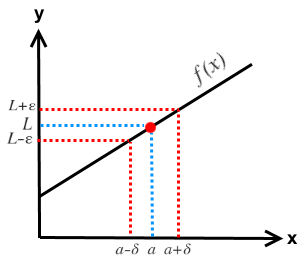
\includegraphics[scale=0.4]{lim}
	\caption{Representação Gráfica - Limite de $f(x)$}
	\label{graflim}
\end{figure}

\end{frame}


\begin{frame}
\frametitle{Propriedades de Limites}
\begin{theorem}[Unicidade do Limite]
	Se $\lim\limits_{x \rightarrow a}f(x) = L_1$ e $\lim\limits_{x \rightarrow a}f(x) = L_2$, então $L_1 = L_2$
\end{theorem}

\pause

\begin{theorem}[Conservação de Sinal]
	Se $\lim\limits_{x \rightarrow a} = L \neq 0$ então existe um intervalo aberto $I$ contendo $a$ tal que, para todo $x \in I \cap D(f)-\{a\}$ tem-se que $f(x)$ possui o mesmo sinal de $L$.
\end{theorem}
\end{frame}


\begin{frame}
\frametitle{Propriedades de Limites}
Se $L$, $M$, $a$ e $k$ são números reais e $\lim\limits_{x \rightarrow a}f(x) = L$ e $\lim\limits_{x \rightarrow a}g(x) = M$ são válidas:
\begin{enumerate}
	\item $\lim\limits_{x \rightarrow a}(f(x) + g(x)) = L + M$
	\item $\lim\limits_{x \rightarrow a}(f(x) - g(x)) = L - M$
	\item $\lim\limits_{x \rightarrow a}(f(x) . g(x)) = L . M$
	\item $\lim\limits_{x \rightarrow a}(k.f(x)) = k.L$
	\item $\lim\limits_{x \rightarrow a}\frac{f(x)}{g(x)} = \frac{L}{M}$, desde que $M \neq 0$
	\item $\lim\limits_{x \rightarrow a}(f(x))^{k} = L^k$, se $k \in \mathbb{Z}$
	\item $\lim\limits_{x \rightarrow a}\sqrt[k]{f(x)} = \sqrt[k]{L}$, se $k \in \mathbb{Z}$ e se $L \geq 0$ quando $k$ é par.
\end{enumerate}
\end{frame}

\begin{frame}
\frametitle{Propriedades de Limites}
\begin{theorem}
	Se $f(x) \leq g(x)$ para todos os valores de $x$ em certo intervalo aberto contendo $a$, exceto possivelmente no próprio $x=a$, e os limites de $f$ e $g$ existem com $x \rightarrow a$, então:
	$$\lim\limits_{x \rightarrow a}f(x) \leq \lim\limits_{x \rightarrow a}g(x)$$
\end{theorem}

\pause

\begin{theorem}[Teorema do Confronto (ou Sanduíche)]
	Se $g(x) \leq f(x) \leq h(x)$ para qualquer $x$ em um intervalo aberto contendo $a$, exceto possivelmente em $x = a$ e $\lim\limits_{x \rightarrow a}g(x) = \lim\limits_{x \rightarrow a}h(x) = L$ então: $\lim\limits_{x \rightarrow a}f(x) = L$
\end{theorem}
\end{frame}

\begin{frame}
\frametitle{Limites Laterais}

\begin{theorem}
	Uma função $f(x)$ terá um limite quando $x$ se aproximar de $a$, sendo $f(x)$ definida na vizinhança de $a$, se e somente se, tiver um limite lateral à direita e um à esquerda, e os dois limites laterais forem iguais:
	$$\lim\limits_{x \rightarrow a}f(x) = L \Leftrightarrow \lim\limits_{x \rightarrow a^{-}}f(x) = \lim\limits_{x \rightarrow a^{+}}f(x) = L$$
\end{theorem}

\end{frame}

\begin{frame}
\frametitle{Limites Infinitos}

\begin{definition}
	Dizemos que $f(x)$ tende ao infinito \emph{ (a menos infinito)} quando $x$ tende a $a$ e escrevemos $\lim\limits_{x \rightarrow a}f(x) = \infty$ \emph{($\lim\limits_{x \rightarrow a}f(x) = - \infty$ )} se para cada número real positivo \emph{(negativo)} $B$ existe um $\delta > 0$ tal que:
	$$0<|x-a|<\delta \Rightarrow f(x) >B $$
	$$0<|x-a|<\delta \Rightarrow f(x) <B $$	
\end{definition}


\end{frame}

\begin{frame}
\frametitle{Limites no Infinito}

\begin{definition}
	Dizemos que $f(x)$ possui limite $L$ quando $x$ tende ao infinito \emph{(menos infinito)} e escrevemos $\lim\limits_{x \rightarrow + \infty}f(x) = L$ \emph{($\lim\limits_{x \rightarrow - \infty}f(x) = L$)} se para cada $\varepsilon > 0$, existe um número $M$ tal que:
	$$x > M \Rightarrow |f(x) - L| < \varepsilon$$
	$$x < M \Rightarrow |f(x) - L| < \varepsilon$$
\end{definition}

\end{frame}

\begin{frame}
\frametitle{Continuidade de Funções}

Uma função é contínua num ponto interior $c$ de seu domínio quando $\lim\limits_{x \rightarrow c}f(x) = f(c)$

\pause

Assim, $f$ será contínua em $c$ se satisfazer:
\begin{enumerate}
	\item $f(c)$ existe $(c \in D(f))$;
	\item $\lim\limits_{x \rightarrow c}f(x)$ existe, ou seja, $\lim\limits_{x \rightarrow c^{-}}f(x) = \lim\limits_{x \rightarrow c^{+}}f(x)$;
	\item $\lim\limits_{x \rightarrow c}f(x) = f(c)$
\end{enumerate}

\end{frame}

\section{REVISÃO - DERIVADAS}

\begin{frame}
\frametitle{Derivadas}
\begin{definition}
	Seja $f$ uma função definida em um intervalo aberto $I$ e $x_0$ um elemento de $I$.
	
	A derivada de $f$ no ponto $x_0$ é o limite, se existir:
	\begin{equation}
	\lim\limits_{x \rightarrow x_0}\frac{f(x) - f(x_0)}{x-x_0}
	\end{equation}
	
	Fazendo $x-x_0=h$ tem-se:
	\begin{equation}
	\lim\limits_{x \rightarrow x_0}\frac{f(x) - f(x_0)}{x-x_0} = \lim\limits_{h \rightarrow 0}\frac{f(x_0 + h)-f(x_0)}{h}
	\end{equation}	
	
	{\bf Notação:} $f'(x_0)$ ou $\dfrac{\partial f}{\partial x} \Big{|}_{x=x_0}$
\end{definition}
\pause

\end{frame}

\begin{frame}
\frametitle{Derivadas}
A derivada nos dá a taxa de variação da função $f$ no ponto $x_0$.

Ou ainda, o coeficiente angular da reta tangente ao gráfico de $f$ no ponto $x=x_0$.
\pause

Se $f$ é uma função derivável em um intervalo, podemos definir a \emph{função derivada} $f'$ que associa a cada $x_0 \in I$ o valor $f'(x_0) = \lim\limits_{x \rightarrow x_0}\frac{f(x) - f(x_0)}{x-x_0}$

\end{frame}

\begin{frame}
\frametitle{Derivadas - Regras de Derivação}

\begin{enumerate}
	\item {\bf Função Constante:} se $f(x) = c$, então $f'(x) = 0$ \pause

	\item {\bf Regra da Identidade:} se $f(x) = x$, então $\dfrac{\partial [x]}{\partial x} = 1$ \pause
	
	\item {\bf Regra da Potência:} se $f(x) = x^n$, então $\dfrac{\partial [x^n]}{\partial x} = nx^{n-1}$ \pause

	\item {\bf  Multiplicação por Constante:} se $w$ é uma função derivável de $x$ e $c$ é uma constante, então $\dfrac{\partial [cw]}{\partial x} = c \dfrac{\partial [w]}{\partial x}$ \pause
    
    \item {\bf Regra da Soma e da Diferença:} $\dfrac{\partial [f(x) \pm g(x)]}{\partial x} = \dfrac{\partial [f(x)]}{\partial x} \pm \dfrac{\partial [g(x)]}{\partial x}$ \pause
    
    \item {\bf Derivada da Exponencial:} $\dfrac{\partial [e^x]}{\partial x} = e^x$ 
    \end{enumerate}
\end{frame}

\begin{frame}
\frametitle{Derivadas - Regras de Derivação}

    \begin{enumerate} \setcounter{enumi}{6}
    \item {\bf Regra do Produto:} $\dfrac{\partial [f(x).g(x)]}{\partial x} = f'(x)g(x)+g'(x)f(x)$, generalizando o caso, segue $\dfrac{\partial [u.v]}{\partial x} = u'.v+u.v'$ \pause
    \item {\bf Regra do Quociente:}$\dfrac{\partial [\frac{f(x)}{g(x)}]}{\partial x} = \frac{f'(x).g(x) - f(x).g'(x)}{[g(x)]^2}$, generalizando o caso, segue que a derivada é dada por $\dfrac{\partial [\displaystyle \frac{u}{v}]}{\partial x} = \displaystyle \frac{u'.v-u.v'}{[v]^2}$ 
    \end{enumerate}


\end{frame}

\begin{frame}
\frametitle{Derivadas - Regra da Cadeia}

A Derivada de funções compostas é obtida através da Regra da Cadeia.

\begin{theorem}[Regra da Cadeia]
	Seja $f(x)$ e $g(x)$ tal que $(g \circ f)(x)$ esteja bem definida. Sendo $f(x)$ derivável em $x$ e $g(x)$ derivável em $f(x)$, a derivada de $(g \circ f)(x)$ é:
	\begin{equation}
	(g \circ f(x))' = (g(f(x)))' = g'(f(x)).f'(x)
	\end{equation}
	Na notação de Leibniz, utilizando $u = f(x)$ e $g(f(x))=g(u)$ temos:
	\begin{equation}
	\dfrac{\partial y}{\partial x} = \dfrac{\partial y}{\partial u} . \dfrac{\partial u}{\partial y}
	\end{equation}
\end{theorem}

\end{frame}

\begin{frame}
\frametitle{Derivadas de Funções Elementares}
\begin{itemize}
 \item Derivada da Função Exponencial: \pause Seja $a \in \mathbb{R}$ tal que $0 < a \neq 1$ e $f(x) = a^x$, então a derivada é: $$y' = a^x .\ln(a)$$ \pause
 Caso particular $a = e$, logo $$ y = e^x \Rightarrow y' = e^x .\ln(e) \Rightarrow y' = e^x $$ \pause


Generalizando: $$y = a^u \Rightarrow y' = a^u.\ln(a).u'$$ $$y = e^u \Rightarrow y' = e^u.u'$$
\end{itemize}


\end{frame}

\begin{frame}
\frametitle{Derivadas de Funções Elementares}
\begin{itemize}
 \item Derivada da Função Logarítmica: \pause Seja $a \in \mathbb{R}$, tal que $0 < a \neq 1$ e $u(x) = \log_{a}x$ sendo que $f^{-1}(x) = u(x)$ e, $f(x) = a^x$, assim a derivada de $u(x)$ é: $$u'(x) = \frac{1}{f'[f^{-1}(x)]}$$ \pause 
 Assim, $$u'(x) = \frac{\log_{a}e}{x}$$ $$u' = \frac{1}{x.\ln(a)}$$

No caso particular que $a = e$ segue: $$u' = \frac{1}{x}$$

\end{itemize}


\end{frame}

\begin{frame}
\frametitle{Derivadas de Funções Elementares}
Generalizando:
$$y = \log_{a}u \Rightarrow y' = \frac{u'}{u.\ln(a)} \text{ ou } y' = \frac{\log_{a}e}{x}$$ 
$$ y = \ln u \Rightarrow y' = \frac{u'}{u}$$

\end{frame}

\begin{frame}
\frametitle{Derivadas - Funções Trigonométricas}
{\bf Algumas Relações Trigonométricas}
$$\tan(x) = \frac{\sin(x)}{\cos(x)}$$
$$\cot(x) = \frac{1}{\tan(x)} = \frac{\cos(x)}{\sin(x)}$$
$$cossec(x) = \frac{1}{\sin(x)}$$
$$\sec(x) = \frac{1}{\cos(x)}$$

{\bf Uma Relação Fundamental}
$$\sin^2(x) + \cos^2(x) = 1$$

\end{frame}

\begin{frame}
\frametitle{Derivadas - Funções Trigonométricas}

{\bf Relações Secundárias}
$$\tan^2(x) + 1 = \sec^2(x)$$
$$1 + \cot^2(x) = cossec ^2(x)$$

{\bf Soma do Seno}
$$\sin(a+b) = \sin(a)\cos(b) + \sin(b)\cos(a)$$

As funções $\sin(x)$ e $\cos(x)$ são contínuas e tem derivadas para todo $x$. As derivadas são:
$$\dfrac{\partial [\sin(x)]}{\partial x} = \cos(x)$$
$$\dfrac{\partial [\cos(x)]}{\partial x} = -\sin(x)$$


\end{frame}

\begin{frame}
\frametitle{Derivadas - Função arco seno}
Os símbolos $\sin^{-1}(x)$ e $\arcsin(x)$ significam ``um ângulo cujo seno é um dado número $x$''

$$y = \sin (x) \Leftrightarrow y^{-1} = \arcsin(x)$$
$$y = \cos (x) \Leftrightarrow y^{-1} = \arccos(x)$$
$$y = \tan (x) \Leftrightarrow y^{-1} = \arctan(x)$$

Derivadas:
$$(\arcsin[u(x)])' = \frac{1}{\sqrt{1 - u^2}}.u'$$
$$(\arccos[u(x)])' = - \frac{1}{\sqrt{1 - u^2}}.u'$$
$$(\arctan[u(x)])' = \frac{1}{1+u^2}.u'$$

\end{frame}

\begin{frame}
\frametitle{Derivadas - Funções Hiiperbólicas}
São combinações.
$$\sinh(x) = \frac{e^x - e^{-x}}{2}$$
$$\cosh(x) = \frac{e^x +e^{-x}}{2}$$

Derivadas:
$$(\sinh(x))' = \cosh(x)$$
$$(\cosh(x))' = \sinh(x)$$

\end{frame}

\begin{frame}
\frametitle{Derivadas de Ordem Superior}
Se $y = f(x)$ é uma função derivável, então $f'(x)$ também é uma função. Se $f'$ for derivável teremos $(f')' = f''$ a segunda derivada de $f$.

Notação: $f''(x)$ ou $\dfrac{\partial ^2 f(x)}{\partial x^2}$, generalizando, $f^{n}(x)$ ou $\dfrac{\partial ^{n}f(x)}{\partial x^{n}}$

\end{frame}


\begin{frame}
\frametitle{Derivadas - Aplicações}
Uma função $f$ tem um valor mínimo local (máximo local) em um ponto interior $c$ de seu domínio se $f(x) \geq f(c)$ $(f(x) \leq f(c))$ para qualquer $x$ em uma vizinhança de $c$. \pause

Se $f$ possui um valor máximo ou mínimo local em um ponto $c$ interior de seu domínio e se $f$ é derivável em $c$, então $f'(c) = 0$. O contrário não se aplica. \pause

Um ponto interior do domínio de $f$ tal que $f'$ é zero ou indefinida é chamado \emph{ponto crítico} de $f$.

\end{frame}


\begin{frame}
\frametitle{Derivadas - Aplicações}
{\bf Teste da Primeira Derivada:} \pause Uma função $f(x)$ é crescente nos intervalos em que $f'(x) > 0$ e é decrescente nos intervalos em que $f'(x) < 0$. \pause

{\bf Teste da Segunda Derivada:} O sinal da segunda derivada é usado para decidir se um ponto crítico é ponto de máximo ou de mínimo.

\end{frame}

\begin{frame}
\frametitle{Derivadas - Aplicações}
\begin{theorem}[de Rolle]
	Se $f$ é uma função contínua em $[a,b]$, derivável em $(a,b)$ e $f(a) = f(b)$, então existe ao menos um ponto $x_0 \in (a,b)$ tal que $f'(x_0) = 0$.
\end{theorem}

\pause

\begin{theorem}[do Valor Médio]
	Se $f$ é uma função contínua em $[a,b]$ e derivável em $(a,b)$ então existe ao menos um ponto $x_0 \in (a,b)$ tal que $f'(x_0) = \frac{f(b) - f(a)}{b-a}$
\end{theorem}



\end{frame}


\begin{frame}
\frametitle{Regra de L'Hôpital}

Sejam $f$ e $g$ funções contínuas e deriváveis em um intervalo aberto $I$ contendo $a$ e suponha que $g'(x) \neq 0$ em $I$, se $x \neq a$ e $f(a) = g(a) = 0$. Então:
$$\lim\limits_{x \rightarrow a}\frac{f(x)}{g(x)} = \lim\limits_{x \rightarrow a}\frac{f'(x)}{g'(x)}$$
desde que o limite do lado direito da igualdade exista.

\pause

{\bf ATENÇÃO:} A Regra de L'Hôpital só pode ser aplicada a limites que resultam em formas indeterminadas.


\end{frame}


\begin{frame}
\frametitle{Taxas Relacionadas}
São problemas onde as quantidades variáveis estão relacionadas entre sí.

Considere a função composta $h(x) = f(g(x))$.

Pela Regra da Cadeia, $h'(x) = f'(g(x)).g'(x)$ ou $\dfrac{\partial h}{\partial x} = \dfrac{\partial f}{\partial g} . \dfrac{\partial g}{\partial x}$

\end{frame}

\section{REVISÃO - INTEGRAIS}
\begin{frame}
\frametitle{Integrais definidas}

\begin{definition}[Integral Definida]
	Se $f$ é uma função definida em $a \leq x \leq b$, dividimos o intervalo $[a,b]$ em $n$ subintervalos de comprimentos iguais $\Delta x = \frac{(b-a)}{n}$.
	
	Sejam $a = x_0, x_1, x_2, \dots, x_n = b$ os extremos desses subintervalos de forma $x^{*}_i$ está no $i-esimo$ subintervalo $[x_{i-1},x_i]$.
	
	Então a {\bf Integral Definida} em $[a,b]$ é:
	
	$$\int_{a}^{b}f(x)dx = \lim\limits_{n \rightarrow \infty}\sum_{k=1}^{n}f(x_{k}^{*})\Delta x$$
\end{definition}
\pause

As funções monótonas ou contínuas por partes (incluindo contínuas) são integráveis.

\end{frame}

\begin{frame}
\frametitle{Integrais - Propriedades}

Ao definirmos $\int_{a}^{b}f(x)dx$, consideramos $a<b$.

Se $b<a$, $\Delta x$ mudará de $\displaystyle \frac{b-a}{n}$ para $\displaystyle \frac{a - b}{n}$. Portanto
$$\int_{b}^{a}f(x)dx = - \int_{a}^{b}f(x)dx$$
Se $a=b$ então $\Delta x = 0$, logo  
$$\int_{a}^{b}f(x)dx = 0$$

\end{frame}

\begin{frame}
\frametitle{Integrais - Propriedades}
{\bf Outras propriedades:}
\begin{enumerate}
	\item $\displaystyle \int_{a}^{b}cdx = c(b-a)$
	\item $\displaystyle \int_{a}^{b}(f(x) \pm g(x))dx = \displaystyle \int_{a}^{b}f(x)dx \pm \displaystyle \int_{a}^{b}g(x)dx$
	\item $\displaystyle \int_{a}^{b}cf(x)dx = c\displaystyle \int_{a}^{b}f(x)dx$
	\item $\displaystyle \int_{a}^{c}f(x)dx + \displaystyle \int_{c}^{b}f(x)dx = \displaystyle \int_{a}^{b}f(x)dx$
\end{enumerate}

\end{frame}

\begin{frame}
\frametitle{Integrais - Propriedades Comparativas}
Vamos supor que $a<b$. Então:
\begin{enumerate}
	\item Se $f(x) \geq 0$ para $a \leq x \leq b$, então $\displaystyle \int_{a}^{b}f(x)dx > 0$
	\item Se $f(x) \geq g(x)$ para $a \leq x \leq b$, então $\displaystyle \int_{a}^{b}f(x)dx \geq \displaystyle \int_{a}^{b}g(x)dx$
	\item Se $m \leq f(x) \leq M$ para $a \leq x \leq b$, então
	$m(b-a) \leq \displaystyle \int_{a}^{b}f(x)dx \leq M(b-a)$
\end{enumerate}

\end{frame}

\begin{frame}
\frametitle{Integrais - Diferenciais}

Seja $y = f(x)$ uma função derivável. A \emph{diferencial $dx$} é uma variável independente. A \emph{diferencial $dy$} é:
$$dy = f'(x)dx$$
Assim, $dy / dx = f'(x) = \displaystyle \frac{dy}{dx}$

\end{frame}

\begin{frame}
\frametitle{Teorema Fundamental do Cálculo}
\begin{lemma}
	Se duas funções $f(x)$ e $g(x)$ possuem a mesma derivada $f'(x) = g'(x)$, então elas diferem por uma constante, ou seja, existe $c \in \mathbb{R}$ tal que $f(x) = g(x) + c$
\end{lemma}

\pause

O Teorema Fundamental do Cálculo nos dará uma relação entre derivadas e integrais.

Seja $f:[a,b] \rightarrow \mathbb{R}$ contínua e $g:[a,b] \rightarrow \mathbb{R}$ definida por $g(x) = \int_{a}^{x}f(t)dt$

\end{frame}

\begin{frame}
\frametitle{Teorema Fundamental do Cálculo}
\begin{theorem}[Fundamental do Cálculo]
	Seja $f$ contínua em $[a,b]$, então:
	\begin{enumerate}
		\item A função $g:[a,b] \rightarrow \mathbb{R}$ definida por $g(x) = \int_{a}^{x}f(t)dt$ $(a \leq x \leq b)$ é contínua em $[a,b]$ e derivável em $(a,b)$ e $g'(x) = F(x)$
		\item Dado $x \in [a,b]$,
		$$\int_{a}^{x}f(t)dt = F(x) - F(a)$$ onde $F$ é qualquer função tal que $F' = f$ ($F$ é primitiva de $f$)
	\end{enumerate}
\end{theorem}


\end{frame}

\begin{frame}
\frametitle{Integrais Indefinidas}
O conjunto de todas as primitivas da função é denominado \emph{integral indefinida de $f$ em relação a $x$} e é denotado por 
$$\int f(x)dx$$
\pause

Este será representado por uma função (uma primitiva de $f$) mais uma constante arbitrária, considerando que duas primitivas quaisquer de $f$ diferem por uma constante.

\end{frame}

\begin{frame}
\frametitle{Integrais - Regra da Substituição}

Seja $u=g(x)$. Pela regra da cadeia, se $F$ é uma primitiva de $f$, então
$$\dfrac{\partial[F(g(x))]}{\partial x} = f(g(x))g'(x)$$
e
$$\int f(u)du = F(u) + c$$
Logo
$$\int f(g(x))g'(x)dx = \int f(u)du$$

Observe que $g'(x)dx = du$, o que pode ser obtido com:
\begin{eqnarray*}
u & = & g(x) \\
\dfrac{\partial u}{\partial x} & = & g'(x) \\
\partial x g'(x) & = & \partial u
\end{eqnarray*}

\end{frame}

\begin{frame}
\frametitle{Integrais - Cálculo de Áreas}

Se $f(x) \geq g(x)$ em $[a,b]$, a área da região entre as curvas $y = f(x)$ e $y = g(x)$ de $a$ até $b$ é a integral de $(f-g)$ desde $a$ até $b$:
$$A = \int_{a}^{b}[f(x)-g(x)]dx$$

\end{frame}

\begin{frame}
\frametitle{Integrais - $\log$}

O logaritmo natural de um número positivo $x$ é 
$$\ln(x) = \int_{1}^{x}\frac{1}{t}dt$$

O número $e$ é o número no domínio do logaritmo natural cuja imagem é $1$, ou seja,
$$\ln(e) = \int_{1}^{e}\frac{1}{t}dt = 1$$ \pause

Pelo Teorema Fundamental do Cálculo, temos $$\dfrac{\partial [\ln(x)]}{\partial x} = \dfrac{\partial\left[ \displaystyle \int_{1}^{x}\displaystyle \frac{1}{t}dt\right]}{\partial x} = \displaystyle \frac{1}{x}$$

\end{frame}


\begin{frame}
\frametitle{Integrais - $\log$}

Como a derivada é sempre positiva, o logaritmo natural é uma função crescente. Logo, é injetora e tem uma inversa. \pause

Ainda, $\dfrac{\partial [\ln(bx)]}{\partial x} = \frac{1}{bx}b = \frac{1}{x}$ onde $b$ é constante qualquer não nula. \pause

Em particular, $\dfrac{\partial [\ln(-x)]}{\partial x} = \frac{1}{x}$

Portanto, para qualquer $x \in \mathbb{R}, x \neq 0$
$$\dfrac{\partial [\ln|x|]}{\partial x} = \frac{1}{x}$$
e
$$\int\frac{1}{u}du = \ln|u| + c$$

\end{frame}


\begin{frame}
\frametitle{Integrais - Técnicas de Integração}

\begin{itemize}
 \item Separando frações; \pause
 \item Reduzindo uma Fração Imprópria; \pause
 \item Completando o quadrado; \pause
 \item Utilizando Identidades Trigonométricas; \pause
 \item Multiplicando por uma forma de $1$; \pause
 \item Através de Frações Parciais;
\end{itemize}


\end{frame}


\begin{frame}
\frametitle{Integrais - Integração por Partes}
Sejam $u$ e $v$ funções deriváveis de $x$. A regra do produto diz que:
\begin{eqnarray*}
(uv)' & = & u'v + uv' \\
\dfrac{\partial [uv]}{\partial x} & = & \dfrac{\partial u}{\partial x}v + \dfrac{\partial v}{\partial x}u \\
\partial[uv] & = & \partial u v + \partial v u \\
uv & = & \int v du + \int u dv \\
\int u dv & = & uv - \int v du
\end{eqnarray*} \pause

Assim, obtemos a fórmula da integração por partes:
$$\int u dv = uv - \int v du$$


\end{frame}


\begin{frame}
\frametitle{Integrais Impróprias}
Vamos atribuir um valor para a área abaixo da curva $y = e^{-\frac{x}{2}}$, $x>0$.
\pause

Primeiro, calculamos a área para $x$ variando de $0$ até $b$, e depois calculamos o seu limite quando $b \rightarrow \infty$.

\begin{eqnarray*}
A(b) & = & \int_{0}^{b}e^{-\frac{x}{2}}dx \\
& = & [-2e^{-\frac{x}{2}}]|_{0}^{b} \\
& = & -2(e^{-\frac{b}{2}}-1) 
\end{eqnarray*}


\end{frame}


\begin{frame}
\frametitle{Integrais Impróprias}

Daí,
\begin{eqnarray*}
\lim\limits_{b \rightarrow \infty}A(b) & = & \lim\limits_{b \rightarrow \infty}(-2(e^{-\frac{b}{2}}-1)) \\
& = & (-2 (0-1)) \\
& = & 2
\end{eqnarray*}
\pause

Podemos escrever:
$$\int_{0}^{\infty}e^{-\frac{x}{2}}dx = \lim\limits_{b \rightarrow \infty}\int_{0}^{b}e^{-\frac{x}{2}}dx$$

\end{frame}


\begin{frame}
\frametitle{Integrais Impróprias}

Generalizando,
$$\int_{a}^{\infty}f(x)dx = \lim\limits_{b \rightarrow \infty}\int_{a}^{b}f(x)dx$$

$$\int_{-\infty}^{b}f(x)dx = \lim\limits_{a \rightarrow - \infty}\int_{a}^{b}f(x)dx$$

Se o limite existe (finito), dizemos que a integral \emph{converge}, caso contrário, dizemos que ela \emph{diverge}.

\end{frame}


\begin{frame}
\frametitle{Integrais Impróprias - Testes de Convergência}

\begin{itemize}
	\item $$\int_{1}^{\infty}\frac{1}{x^p}dx \Rightarrow \begin{cases}
		\text{ converge, se }p > 1 \\
		\text{ diverge, se } p \leq 1
	\end{cases}$$
	\item $$ \int_{1}^{\infty}a^x dx \Rightarrow \begin{cases}
	\text{ converge, se } a < 1 \\
	\text{ diverge, se } a \geq 1
	\end{cases}$$
\end{itemize}
\pause

{\bf Teste da Comparação:} sejam $f$ e $g$ contínuas em $[a,\infty)$, com $0 \leq f(x) \leq g(x) $ para qualquer $x \geq a$. Então:
\begin{enumerate}
	\item $\displaystyle \int_{a}^{\infty}f(x)dx$ converge se $\displaystyle \int_{a}^{\infty}g(x)dx$ converge;
	\item $\displaystyle \int_{a}^{\infty}g(x)dx$ diverge se $\displaystyle \int_{a}^{\infty}f(x)dx$ diverge.
\end{enumerate}


\end{frame}


\begin{frame}
\frametitle{Integrais Impróprias - Testes de Convergência}
{\bf Teste da Comparação no Limite:} se $f$ e $g$ são funções positivas contínuas em $[a,\infty)$ e se
$$\lim\limits_{x \rightarrow \infty}\frac{f(x)}{g(x)} = L, \text{   } 0 < L < \infty$$
então $\displaystyle \int_{a}^{\infty}f(x)dx$ e $\displaystyle \int_{a}^{\infty}g(x)dx$ são ambas convergentes ou ambas divergentes.


\end{frame}

\end{document}

